\chapter{Svolgimento del Tirocinio}

In questo capitolo verrà spiegato nel dettaglio lo svolgimento del tirocinio. L'obiettivo preposto è stato quello di realizzare un'applicazione funzionante per visualizzare e gestire mappe geospaziali. Lo sviluppo si è diviso tra front-end, per consentire la visualizzazione delle mappe, e back-end, per la loro gestione e fornirle al primo. Parte del codice si è inoltre focalizzata sulla comunicazione tra front-end e back-end.

\section{Preparazione al Tirocinio}

\subsection{Studio di Reactive Programming e Angular}
I primi giorni di tirocinio sono stati dedicati allo studio autonomo dei linguaggi di programmazione e delle librerie utilizzate all'interno del progetto. Particolare attenzione è stata dedicata inizialmente alla parte di sviluppo front-end, dedicando le prime settimane allo studio del framework JavaScript Angular, e al suo corrispettivo linguaggio di programmazione TypeScript.
Lo studio di queste tecnologie è terminato con la realizzazione di un piccolo progetto in Angular 17, che è possibile replicare seguendo la sua documentazione \cite{DocumentazioneAngular}. Si è poi proseguito con lo studio della libreria RxJS, fondamentale per l'uso di Angular, in quanto è parte integrante dello stesso.
Tale libreria viene utilizzata internamente da Angular per gestire numerose operazioni asincrone attraverso l'uso di Stream, adottando il paradigma di "Reactive Programming" invece che "Event Driven".
\\Nel paradigma a eventi, viene scritto del codice per gestire un evento quando questo si verifica. In genere si definisce una funzione, nota come callback, che viene registrata su un certo evento. Quando tale evento si verifica, come ad esempio un click del mouse su un pulsante, la funzione registrata viene invocata per gestire l'evento di click.
Nell'approccio reattivo, invece, viene scritto del codice per gestire uno Stream di dati che rappresenta una sequenza continua di eventi. Ad esempio, invece di gestire il singolo click del mouse, viene creato uno Stream che rappresenta i click che avvengono del tempo. Tale Stream può essere manipolato, filtrato o trasformato utilizzando degli operatori.
\\Angular utilizza RxJS per adottare quest'ultimo tipo di paradigma, facendo uso di tre elementi interdipendenti: l'Observable, gli Operator e gli Observer.
\\L'Observable è colui che fornisce i dati sullo Stream ed è colui che è oggetto dell'osservazione. Durante il fornimento dei dati, che avviene in maniera continua nel tempo, gli Operator si occupano di manipolarli. Gli Operator sono delle operazioni che permettono la manipolazione dei dati sullo Stream in maniera asincrona. Le operazioni più note sono la mappatura, il filtraggio, la combinazione e la trasformazione. L'Observer si trova alla fine della catena e si occupa di utilizzare il risultato dei dati elaborati.
\\Angular utilizza internamente gli Observable a basso livello per gestire i suoi componenti, mentre ne espone un'interfaccia semplificata ad alto livello per l'utilizzo da parte degli sviluppatori. Ad esempio, il routing delle pagine web e il modulo del form di input fanno uso degli Observable per monitorare e rispondere agli eventi di input dell'utente.

% \subsubsection{Primo componente in Angular}

% Il lavoro è poi proseguito con la realizzazione di un piccolo componente in Angular richiesto dall'azienda, al fine di consolidare le competenze acquisite. Il lavoro consisteva nel realizzare delle

% \begin{figure}[htbp]
%     \centering
%     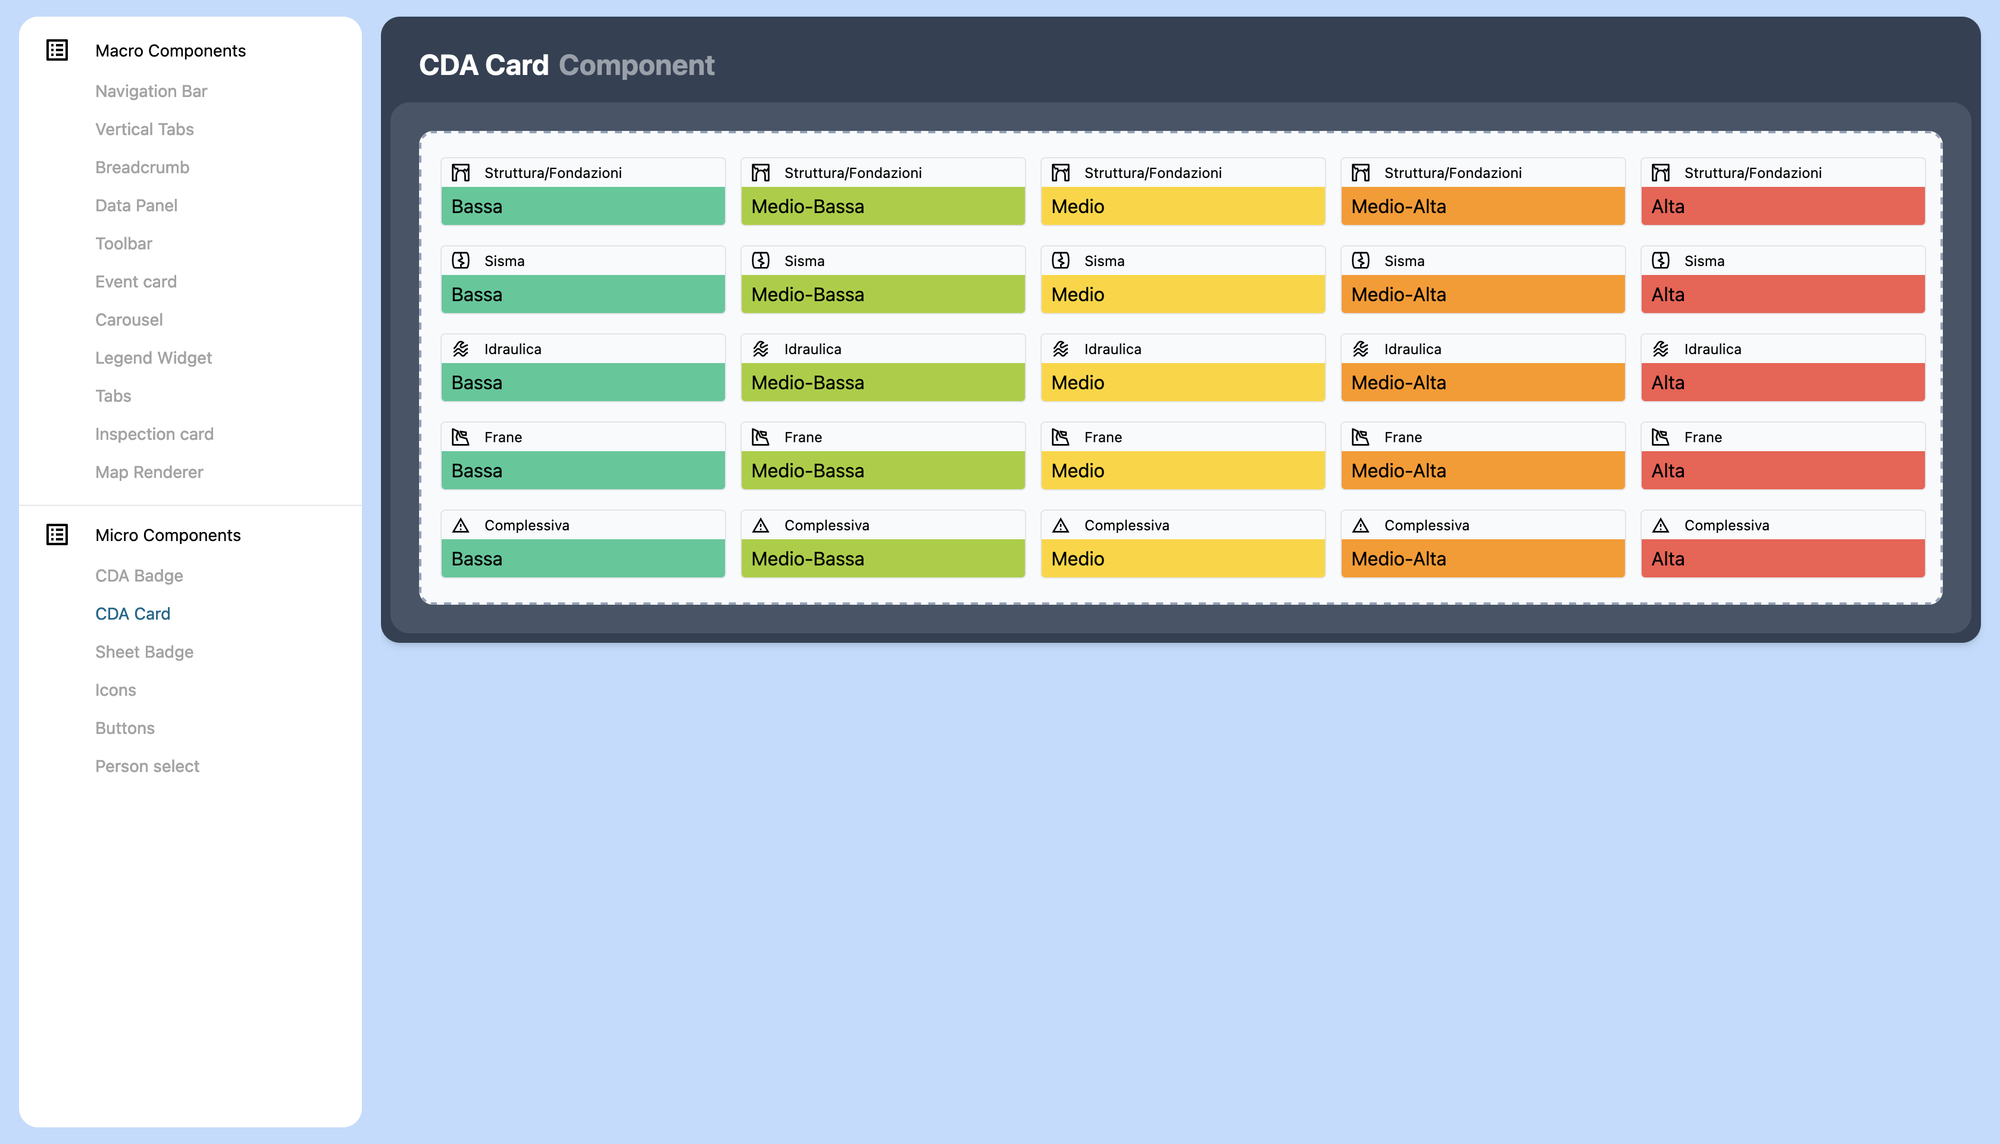
\includegraphics[width=1\textwidth]{images/Capitolo3/CDACardComponent.png}
%     \caption{CDA Card Component}
%     \label{fig:CDA Card Component}
% \end{figure}

\subsection{Realizzazione di un prototipo con OpenLayers}

% vecchio: Al fine di comprendere meglio il suo funzionamento e di semplificarne l'utilizzo, il candidato ha deciso non iniziare direttamente con lo sviluppo del progetto, ma ha proseguito con l'implementazione di una piccola applicazione esterna, priva del framework Angular e librerie di terzi.
Lo sviluppo delle mappe da parte del tirocinante è iniziato con lo studio e l'utilizzo della libreria OpenLayers. Al fine di capirne meglio il suo funzionamento, il candidato ha deciso di non iniziare direttamente con lo sviluppo del progetto di tirocinio, ma ha proseguito con l'implementazione di una piccola applicazione esterna, priva del framework Angular e librerie di terzi, così da semplificarne il suo utilizzo. Come riportato dalla documentazione \cite{DocumentazioneOpenLayersBase}, OpenLayers si basa su quattro componenti principali:

\begin{itemize}
    \item Map: per la manutenzione e revisione del codice;
    \item View per i test test cases, continuous integration e
    \item Source
    \item Layers
\end{itemize}
Qui sotto viene riportato una parte del codice del prototipo, così da comprendere meglio il funzionamento della libreria.
\lstinputlisting[language=html, caption={Codice HTML}]{listings/Capitolo3/index.html}
% \texttt{Codice JavaScript}.
\lstinputlisting[caption={Codice JavaScript}, language=Java]{listings/Capitolo3/main.js}

\subsection{Studio di OpenLayers in Angular}

Il candidato, infine, ha confrontato il suo lavoro con quello già presente all'interno del progetto realizzato in Angular, così da comprendere al meglio le differenze fra le due implementazioni e capire quali funzionalità fossero già state realizzate.
\\La loro versione presentava solamente l'integrazione agli elementi base di OpenLayers, un supporto alla sovrapposizione multipla di layer differenti e un layer di default, che mostrava una mappa di base fornita da OpenStreetMap. La differenza principale, essendo stata realizzata in Angular, è che la loro implementazione era stata fatta tramite l'uso di componenti, in questo modo poteva il componente della mappa poteva essere facilmente importato più volte all'interno delle varie pagine web dell'applicazione.
\\Inizialmente, infatti, tale componente era situato all'interno della pagina web dell'Ui-Kit, ma allo sviluppatore di importare più volte il componente della mappa nell'applicazione. ovvero una pagina contente, a scopo dimostrativo, tutti i componenti grafici che sarebbero stati poi utilizzati all'interno dell'applicazione. L'uso dell'Ui-Kit è una pratica comune, specialmente nel contesto di applicazioni Enterprise, in quanto permette agli sviluppatori.
\\Ovviamente l'uso dell'Ui-Kit è reso possibile grazie ai framework JavaScript come Angular, la cui architettura modulare rende possibile l'esportazione dei componenti creati in altre pagine web dell'applicazione. Ad esempio, quando uno sviluppatore crea un componente nell'Ui-Kit, può facilmente importarlo e utilizzarlo all'interno delle varie pagine del sito, senza doverlo ricreare da zero ogni volta. Senza Angular, questa operazione sarebbe molto più laboriosa, dovendo riscrivere più volte lo stesso codice e quindi non risulterebbe più conveniente.

% L'UI Kit è utile perché fornisce una libreria di componenti grafici predefiniti che consentono agli sviluppatori di mantenere la coerenza visiva e funzionale nell'interfaccia utente dell'applicazione. Utilizzandolo, si risparmia tempo evitando di dover progettare e implementare ogni elemento da zero. Inoltre, offre la possibilità di personalizzare i componenti per adattarli alle esigenze specifiche del progetto, garantendo una migliore integrazione e flessibilità nel processo di sviluppo.

% L'UiKit è una pratica comune, specialmente all'interno di applicazioni Enterprise, in quanto offre diversi vantaggi come l'aiuto agli sviluppatori front-end ad avere una base solida ed uniforme dell'interfaccia utente

% ia dal punto di vista della programmazione, in quanto aiuta gli sviluppatori front-end ad avere una base solida ed uniforme di progettazione dell'interfaccia utente,

% sia perché funge da strumento di presentazione del design ai potenziali clienti, consentendo loro di visualizzare in anteprima l'aspetto e le funzionalità dell'applicazione

% Inoltre, l'utilizzo dell'UiKit favorisce l'efficienza nello sviluppo. Gli sviluppatori possono ridurre il tempo necessario per progettare e implementare nuove funzionalità dell'interfaccia utente, poicheé angular. Questo permette di accelerare il processo di sviluppo e di ridurre i costi associati.
% Infine, l'UiKit favorisce la manutenibilità del codice. Poiché i componenti dell'interfaccia utente sono riutilizzabili e modulari, è più semplice apportare modifiche e aggiornamenti all'interfaccia utente senza dover modificare il codice sorgente in più punti. Questo rende più agevole la gestione e l'evoluzione dell'applicazione nel tempo, garantendo una maggiore flessibilità e scalabilità.

% fornire una base consistente per la progettazione dell'interfaccia utente,
% bibop
% L'obiettivo principale di un UI kit è quello di fornire una base consistente per la progettazione e lo sviluppo dell'interfaccia utente, facilitando così il lavoro degli sviluppatori e garantendo una migliore coerenza visiva e funzionale nell'applicazione finale. Utilizzando un UI kit, gli sviluppatori possono risparmiare tempo nella progettazione e implementazione dell'interfaccia utente, concentrandosi invece sulle funzionalità e sull'esperienza utente dell'applicazione.

\subsection{Censimento delle Mappe}

Il tirocinio è poi continuato con lo studio e alla comprensione dei protocolli OGC e dei concetti fondamentali relativi ai dati geospaziali. In particolare, l'attenzione è stata concentrata sui protocolli WMS (Web Map Service) e WFS (Web Feature Service), poiché sono tra i più utilizzati e facili da distinguere. Questo ha permesso di comprendere al meglio il loro funzionamento e le principali differenze tra essi. Per quanto concerne i dati geospaziali, invece, lo studio si è dedicato principalmente ai formati GeoJSON e Shapefile, in quanto sono anch'essi formati geospaziali comuni e ampiamente utilizzati.
\\Dopo questa fase di apprendimento iniziale, il candidato ha collaborato con l'azienda per identificare le fonti da cui raccogliere le mappe necessarie, censendole in un documento dettagliato. Questo processo ha permesso di avere una panoramica completa delle risorse geospaziali disponibili e di comprendere meglio come organizzarle e utilizzarle nel contesto del mio tirocinio. Le mappe utilizzate all'interno del progetto provengono principalmente da tre fonti:
\begin{itemize}
    \item \textit{Geoportale Nazionale}, un portale gestito dal Ministero dell'Ambiente e della Sicurezza Energetica che contiene dati geospaziali forniti tramite protocollo OGC, quali WMS, WFS e WCS. É possibile reperire le mappe utilizzate dal loro sito \cite{GeoPortaleNazionale}.
    \item \textit{IdroGEO}, una piattaforma gestita ISPRA (Istituto Superiore per la Protezione de la Ricerca Ambientale), che permette agli utenti di accedere e di scaricare dati di mappe, in formato Shapefile o GeoJSON, relativi al rischio idrogeologico in Italia. Precisamente fornisce informazioni sull'Inventario dei Fenomeni Franosi in Italia (IFFI), e sulle mappe nazionali di pericolosità da frane e alluvioni e sugli indicatori di rischio associati.
    \item \textit{GeoCart}, un'azienda italiana specializzata nella produzione e distribuzione di mappe e prodotti cartografici \cite{GeoCart}. Anche in questo caso le mappe sono in formato Shapefile, ma a differenza di quelle precedenti, non sono di dominio pubblico e non sono accessibili in modo gratuito. Sono risorse sviluppate ai fini commerciali.
\end{itemize}

\section{Sviluppo Front-end con OpenLayers}

\subsection{Perché OpenLayers}

Tale libreria è stata scelta, rispetto alle altre concorrenti, in quanto offre internamente molte funzionalità utili per la rappresentazione di questo tipo di mappe.
\\Come già spiegato nel secondo capitolo, OpenLayers offre un supporto già integrato ai protocolli OGC, essenziali per la rappresentazione di questi tipi di dati geospaziali. La maggior parte delle sorgenti di mappe fornite, infatti, sono trasmesse mediante protocolli OGC quali WMS, WFS e WCS. Con l'utilizzo di questa libreria, la comunicazione ai servizi OGC esterni risulta essere più semplice, in quanto non è necessario eseguire manualmente tutte le richieste imposte dallo Standard, e, successivamente, eseguire il parsing sul contenuto delle risposte in formato XML. OpenLayers fornisce, a più livelli, delle classi che si occupano di eseguire queste operazioni al posto nostro, e attraverso il principio di Information Hiding, espongono allo sviluppatore solo il minimo necessario per eseguire correttamente la richiesta.
\\Per esempio, nel caso dell'implementazione del protocollo WMS, non sarà quindi necessario eseguire una richiesta di GetCapabilities e successivamente GetMap, al fine di ricevere l'immagine della mappa. Se il nome del layer è noto, basterà istanziare la classe ImageWMS che passandogli i parametri corretti, eseguirà automaticamente le operazioni necessarie al fine di ricevere l'immagine della mappa corretta. Qui sotto viene riportato un esempio di implementazione della classe ImageWMS, il quale è possibile reperire anche dalla documentazione di OpenLayer\cite{DocumentazioneOpenLayersWMS}
\lstinputlisting[language=Java, caption={Esempio di ImageWMS}]{listings/Capitolo3/openLayerWMS.js}
Come si può vedere dall'esempio, al fine di recuperare l'immagine della mappa fornita dal server WMS esterno, è necessario istanziare la classe ImageWMS passandogli come argomento soltanto l'URL e il layer che si vuole visualizzare.
OpenLayer si occuperà di eseguire la richiesta di GetMap al posto nostro e di mostrare a schermo l'immagine della mappa.
\\Tale esempio richiede ovviamente che il nome del layer sia noto, nel caso in cui il client non conosca la lista di layer disponibili, sarà comunque necessario eseguire una richiesta di GetCapabilities.
\\Anche in questo caso, OpenLayer si occupa di eseguire la richiesta e di effettuare il parsing in automatico sul contenuto dell'XML, senza dover creare una struttura dati apposita per manipolare i dati ricevuti da essa.
\lstinputlisting[language=Java, caption={Esempio di GetCapabilities per WMS}]{listings/Capitolo3/openLayerWMSCapabilities.js}
Inoltre la libreria ha già un supporto integrato per il formato GeoJSON, il che la rende ottimale al fine di testare le mappe fornite da IdroGEO, in quanto quest'ultime non vengono distribuite mediante un servizio OGC, ma vengono fornite come file locali in formato GeoJSON.
\\Infine, la libreria è interamente supportata da Angular e con un semplice comando di npm (mpm install ol), la si può installare all'interno del progetto, il che la rende ottimale per questo tipo di applicazione.

% poi spiego come ho fatto l'applicazione
% poi spiego i problemi come li ho affrontati (pro4j, geojson)

\subsection{Implementazione nel Progetto}

Il candidato, sotto supervisione del tutor aziendale, ha iniziato lo sviluppo del progetto BMS creando all'interno dell'applicazione una nuova pagina web, nella quale ha importato il componente della mappa già esistente nell'Ui-Kit, così da poter integrare il supporto ai protocolli OGC richiesti e iniziare a testare le mappe censite.
\\Lo sviluppo è proseguito estendendo il componente Angular delle mappe, che fino a quel momento ha presentato solamente l'integrazione agli elementi base di OpenLayers e un supporto alla sovrapposizione multipla di layer differenti.
\\Come prima funzionalità si è implementato il supporto al formato GeoJSON, selezionando come prima mappa da testare quella delle frane in Toscana, fornita da IdroGEO, in quanto tutte quelle fornite da questo ente, possono essere scaricate localmente e caricate all'interno del progetto, senza dover contattare alcun servizio esterno. Ciò facilità il lavoro di programmazione, riducendo il rischio di errore dovuto a eventuali problemi di disservizio dei server di mappe esterni.
\\In questa fase, le parti di codice che hanno subito più modifiche sono le classi BuildLayer.ts e MapModel.ts, le quali si occupano di far istanziare l'oggetto della mappa con proprietà differenti, in base al tipo di formato geospaziale passato come argomento.
\\Il lavoro è continuato con l'implementazione della pagina web descritta precedentemente, andando a inserire al suo interno alcune mappe fittizie, tra cui una in formato GeoJSON, così da poterne verificare il funzionamento. Tali mappe, rappresentate come "layer", sono state tutte sovrapposte a quella di default, ovvero quella di OpenStreetMap. In questo modo si è compreso se i layer sono stati rappresentati correttamente, riuscendo così a orientarsi all'interno delle mappe stesse in termini geografici.


spiegare openstreet map
voglio dire che ho aggiunto il layer di openstreet map
voglio dire del problema di pro4j
voglio dire del problema di clustering e la ram mangiata
voglio dire dello stile applicato e il click dei marker


\lstinputlisting[language=Java, caption={Implementazione BuildLayer}]{listings/Capitolo4/buildLayer.js}




% in questa fase il lavoro si è prevalentemente incentrato sulla classe BuildLayer.ts, la quale si occupa di bababababab. Alla seguente classe sono stato apportate le seguenti modifiche: basdbsamdasbdnas


% * oh no! non va na sega! usiamo pro4j *





% è stato scelta una mappa di IdroGEO in formato geojson, perché


% Abbiamo preso i link dei dati delle mappe che ho censito i primi giorni. Abbiamo scelto un link del sito blu (quello idrico) e abbiamo provato a prendere il file delle frane della toscana in formato GeoJson e darlo in pasto a open layer, nella speranza che in automatico riuscisse a capire quei dati e mostrarli a schermo.
% Abbiamo quindi creato un nuovo tipo e fornito nella condizione dello switch case iniziato da Alessandro (lui aveva fatto funzionare i tipi: assets, tiles, topojson, ma non geojson!)
% Abbiamo creato un nuovo layer con new GeoJson() supportato direttamente da open layer.
% Abbiamo definito lo stile in cui i dati nel file geojson dovevano essere rappresentati (dei cerchi rossi in svg).
% A quanto pare il formato geojson serve per disegnare roba nella mappa, come coordinate punti o linee, non mappe. Di conseguenza ci serve uno stile da dare a open layer con cui deve leggere.
% A questo punto abbiamo fatto renderizzare la mappa a schermo ma senza successo. Il codice era scritto correttamente ma il sistema di coordinate passato dal file geojson era sconosciuto a open layer.
% Quindi abbiamo creato una nuova projection con le chiamate fornite della libreria e abbiamo definito il funzionamento di quella projection con una libreria chiamata `proj4`.
% Questa libreria permette di fare in automatico il cambio di coordinate da un sistema di riferimento ad un altro. Quindi e’ bastato fare la conversione e dare il risultato ad open layer.
% Poiche’ il file era di 64 Mega, e la quantita’ di dati era cosi densa, la mappa e’ arrivata a consumare la bellezza di 27 GB di ram prima di andare poi in swap e crashare. Quindi e’ stato necessario ‘clasterizzare’ i dati. Fortunatamente anche qui, open layer ci da una mano con una funzione cluster

% proiezione con pro4j,




% \section{Questa è una sezione}

% \lipsum[2]

% \subsection{Questa è una aaaaaa}

% \lipsum[3]

% \subsubsection{Questa è una sotto-sottosezione}

% \lipsum[4]

% É possibile riferire l'immagine, una volta assegnatagli una label, tramite il comando \texttt{\textbackslash autoref\{fig:immagine\}}, ottenendo il seguente risultato: \autoref{fig:immagine}.

% \begin{figure}
%     \centering
%     
\includegraphics[width= 0.8\textwidth]{images/Capitolo1/immagine.jpg}
%     \caption{Questa è un'immagine}
%     \label{fig:immagine}
% \end{figure}

% Questa è una citazione \cite{LabelPerLaCitazione}.

% \subsubsection{Questa è un'altra sottosezionelipsum}

% Quello che segue è un esempio di codice. E' possibile modificare il linguaggio per il synyax highlight, aggiungere parole chiave... E' tutto disponibile nella guida del pacchetto \texttt{listings}.

% \lstinputlisting[language=C++]{listings/Capitolo1/code1.cpp}

% \section{Questa è un'ennesima sezione}

% \lipsum[4]

% \subsection{Sottosezione con una tabella}

% La tabella si indirizza sempre con l'uso di una label, ottenendo il risultato \autoref{tab:labelTabella}.

% \begin{table}
%     \caption{Una simpatica tabella!}\label{tab:labelTabella}
%     \begin{center}
%         \begin{tabular}{c|c|c|c}
%             \textbf{Colonna 1} & \textbf{Colonna 2} & \textbf{Colonna 3} & \textbf{Colonna 4} \\
%             \hline
%             $3$                & $24$               & $24$               & $29$               \\
%             $36$               & $31$               & $49$               & $39$               \\
%             $32$               & $41$               & $59$               & $57$               \\
%             $34$               & $60$               & $79$               & $74$               \\
%             $328$              & $96$               & $194$              & $99$               \\
%             $356$              & $117$              & $297$              & $149$              \\
%             $312$              & $315$              & $293$              & $242$              \\
%             $3024$             & $184$              & $253$              & $019$              \\
%             $3048$             & $7795$             & $253$              & $077$              \\
%             $3096$             & $7767$             & $2432$             & $0514$             \\
%             $3192$             & $3769$             & $2435$             & $0551$             \\
%             $36384$            & $6625$             & $3432$             & $0497$             \\
%             $32768$            & $15469$            & $6472$             & $0471$             \\
%             $35536$            & $15425$            & $14539$            & $10289$            \\
%             $331072$           & $34623$            & $24941$            & $20444$            \\
%         \end{tabular}
%     \end{center}
% \end{table}